\section{Parte 2: el calendario}
\label{sec:parte2}

La serie se construye en \texttt{calendario.py}: se suma
$\texttt{Quantity}\times\texttt{UnitPrice}$ por día sobre los datos de
\texttt{limpiar(df)} (reglas 1 a 5, con cancelaciones restando y con las
ventas sin cliente) y se lleva al calendario completo. Las tablas y figuras de
esta sección las genera \texttt{parte2.py}.

\subsection{Inciso 2.1: la serie de venta neta diaria}

\begin{table}[H]
  \centering
  \small
  \tabla{p2_resumen}
  \caption{Días calendario y días con transacciones.}
  \label{tab:p2_resumen}
\end{table}

Entre el 1 de diciembre de 2010 y el 9 de diciembre de 2011, contando ambos,
hay 374 días calendario, y en 305 hubo al menos una transacción
(tabla~\ref{tab:p2_resumen}). Es decir, en 69 días (el 18\%) la tienda no
registró nada. La figura~\ref{fig:p2_serie} muestra la serie en los días
abiertos. Los cierres entre semana están marcados con una cruz sobre el eje;
los sábados no se marcan porque ocurren todas las semanas.

\begin{figure}[H]
  \centering
  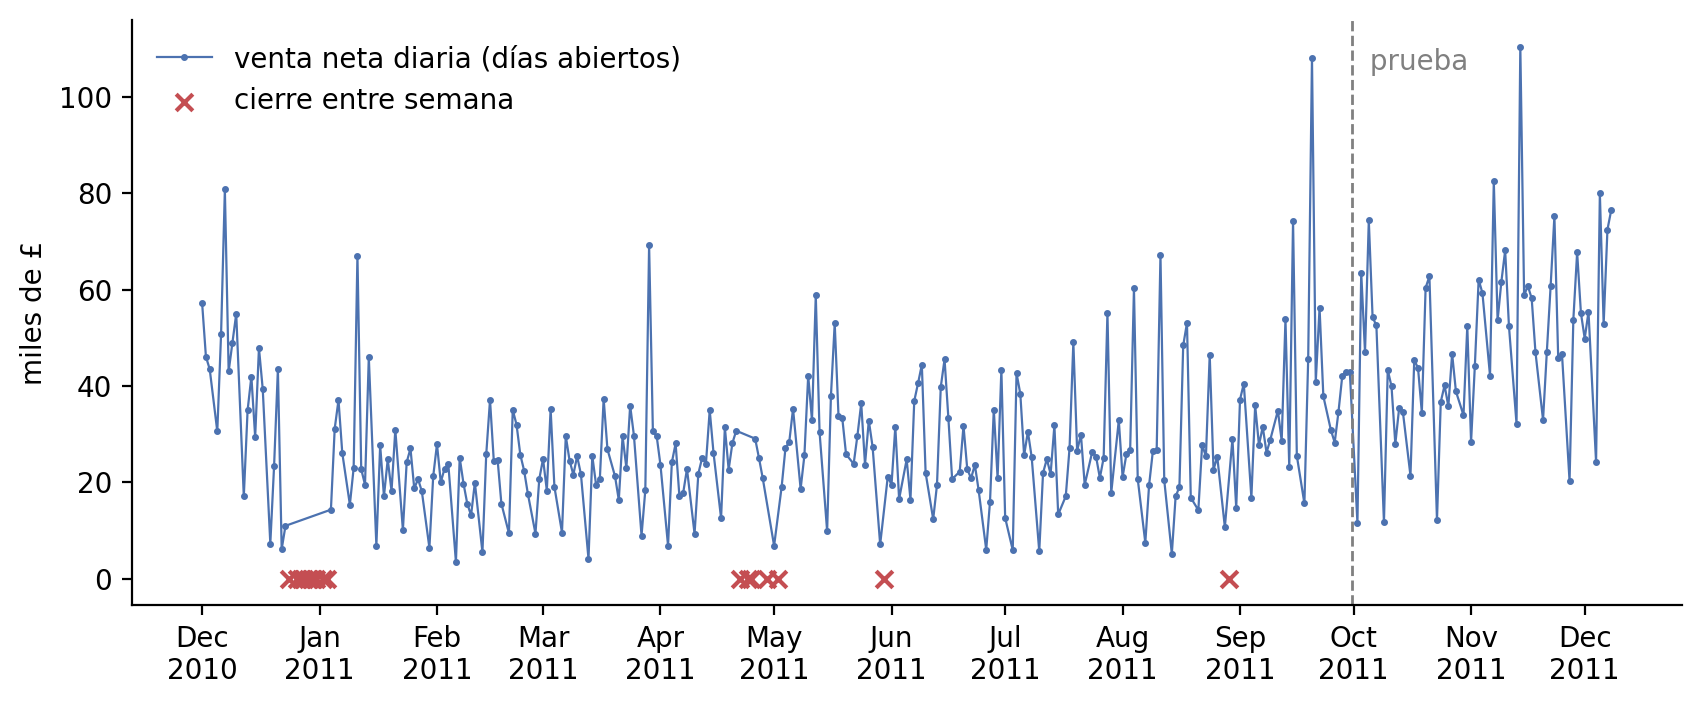
\includegraphics[width=\textwidth]{p2_serie_diaria.png}
  \caption{Venta neta diaria en los días abiertos, del 1 de diciembre de 2010
  al 8 de diciembre de 2011. La línea une días abiertos consecutivos, así que
  salta por encima de los sábados y de los cierres. La línea punteada separa
  el entrenamiento (hasta el 30 de septiembre) de la prueba.}
  \label{fig:p2_serie}
\end{figure}

La figura ya anticipa lo que se va a modelar en las siguientes partes: un
nivel de alrededor de \pounds20--30 mil diarios entre enero y agosto, un
crecimiento fuerte desde septiembre (la temporada navideña de una tienda de
regalos que vende a mayoristas) y mucha variación de un día a otro, con picos
aislados de más de \pounds100 mil.

\subsection{Inciso 2.2: los días sin transacciones}

\paragraph{Los sábados.} 53 de los 69 días faltantes son sábados: \emph{todos}
los sábados del periodo. No hay ni una sola transacción en sábado en todo el
año, así que la tienda no abre ese día. En cambio sí abre los domingos.

\paragraph{Los otros 16.} La tabla~\ref{tab:p2_cierres} los lista y los
clasifica usando el calendario de \emph{bank holidays} de Inglaterra y Gales.

\begin{table}[H]
  \centering
  \small
  \tabla{p2_cierres}
  \caption{Días entre semana (sin contar sábados) sin ninguna transacción.}
  \label{tab:p2_cierres}
\end{table}

\begin{itemize}
  \item \textbf{Cierre de Navidad: 9 días}, del viernes 24 de diciembre de
    2010 al lunes 3 de enero de 2011. En 2010 Navidad cayó en sábado y el
    \emph{Boxing Day} en domingo, así que los feriados oficiales se
    trasladaron al lunes 27 y al martes 28; Año Nuevo de 2011 cayó en sábado
    y se trasladó al lunes 3 de enero. Los días que quedan en medio (29, 30 y
    31 de diciembre y el domingo 2 de enero) no son feriados oficiales: la
    tienda simplemente cerró entre fiestas, algo común en un negocio que le
    vende a otros negocios.
  \item \textbf{Pascua: 3 días}, el Viernes Santo (22 de abril), el Domingo de
    Pascua (24 de abril) y el Lunes de Pascua (25 de abril). El domingo no es
    feriado oficial, pero la tienda, que sí abre otros domingos, no abrió
    entre los dos feriados.
  \item \textbf{La boda real: 1 día}, el viernes 29 de abril de 2011, el
    matrimonio del príncipe Guillermo con Catalina Middleton. Es el feriado
    que no se repite: el gobierno lo declaró solo para ese año.
  \item \textbf{Feriados de lunes: 3 días}, el \emph{Early May bank
    holiday} (2 de mayo), el \emph{Spring bank holiday} (30 de mayo) y el
    \emph{Summer bank holiday} (29 de agosto).
\end{itemize}

Todos los feriados oficiales del periodo aparecen como días sin ventas, y
fuera de los sábados no falta ningún otro día: no hay caídas del sistema ni
días perdidos sin explicación.

\paragraph{¿Cuáles son móviles?} Los de Pascua. La Pascua cae el primer
domingo después de la primera luna llena de primavera, así que el Viernes
Santo puede caer en cualquier fecha entre el 20 de marzo y el 23 de abril, y
el Lunes de Pascua tres días después: de un año a otro se mueven hasta cinco
semanas. Por eso
FPP2 dice que son de lo más difícil de modelar con datos diarios: un modelo
con estacionalidad de 7 días o de 365 días no los puede anticipar, porque no
caen a una distancia fija de nada. Los tres feriados de lunes también cambian
de fecha de un año a otro, pero siguen una regla de calendario sencilla
(primer o último lunes del mes), siempre caen en lunes y se conocen con años de
anticipación. La Navidad tiene fecha fija, pero el día de la semana cambia y
con él los traslados, como pasó en 2010. La boda real no se puede modelar con
ningún patrón, porque solo ocurrió una vez.

\subsection{Inciso 2.3: ¿cero o faltante?}

Un día sin transacciones puede ser cualquiera de las dos cosas; depende de
para qué se use la serie.

\paragraph{Cuándo es un cero.} Cuando la pregunta es contable, como cuánto
vendió la tienda en una semana o en un mes, o cuál es la venta promedio por
día calendario. El sábado la caja recibió exactamente cero libras, y sumar la
serie con ceros da el total correcto. Es el uso de la media móvil del inciso
3.1, donde el enunciado pide rellenar con cero: una semana con un feriado sí
vendió menos que una semana normal, y la tendencia debe reflejarlo.

\paragraph{Cuándo es un faltante.} Cuando se modela el comportamiento de la
tienda en los días en que opera: los índices estacionales, la ACF, los
modelos AR y SARIMA y la evaluación del pronóstico. Ahí un cero de sábado no
es una observación de ``un día malo'': no hubo ningún día que observar. Si se
deja como cero, el índice estacional del sábado sería cero (algo que ya se
sabe y no hay que estimar); la media de la serie bajaría un 18\% (69 de 374 días);
aparecería un $r_7$ enorme que no viene de la demanda sino del calendario; y
un pronóstico que acierte ``cero'' cada sábado se vería artificialmente bueno.
Por eso, de aquí en adelante, la serie tiene los días cerrados como faltantes
y los modelos trabajan con una fila por día abierto.

\subsection{Inciso 2.4: el último día}

El 9 de diciembre de 2011 no está completo. Su última factura es de las 12:50
y suma \pounds29\,306 en 49 facturas, cuando un viernes de noviembre o
diciembre vende una mediana de \pounds52\,410. Ningún día anterior del año
registró su última factura antes de las 12:50: los datos se cortaron a
mediodía, probablemente cuando se extrajo el archivo.

Se puede medir qué tan incompleto está. Para cada viernes anterior se calculó
qué fracción de sus ventas se había registrado a las 12:50
(figura~\ref{fig:p2_corte}). La mediana es 54\%, así que el 9 de diciembre
completo habría vendido alrededor de $29\,306/0.54\approx$ \pounds54\,200, en
línea con los viernes anteriores. Es decir, al día le falta casi la mitad.

\begin{figure}[H]
  \centering
  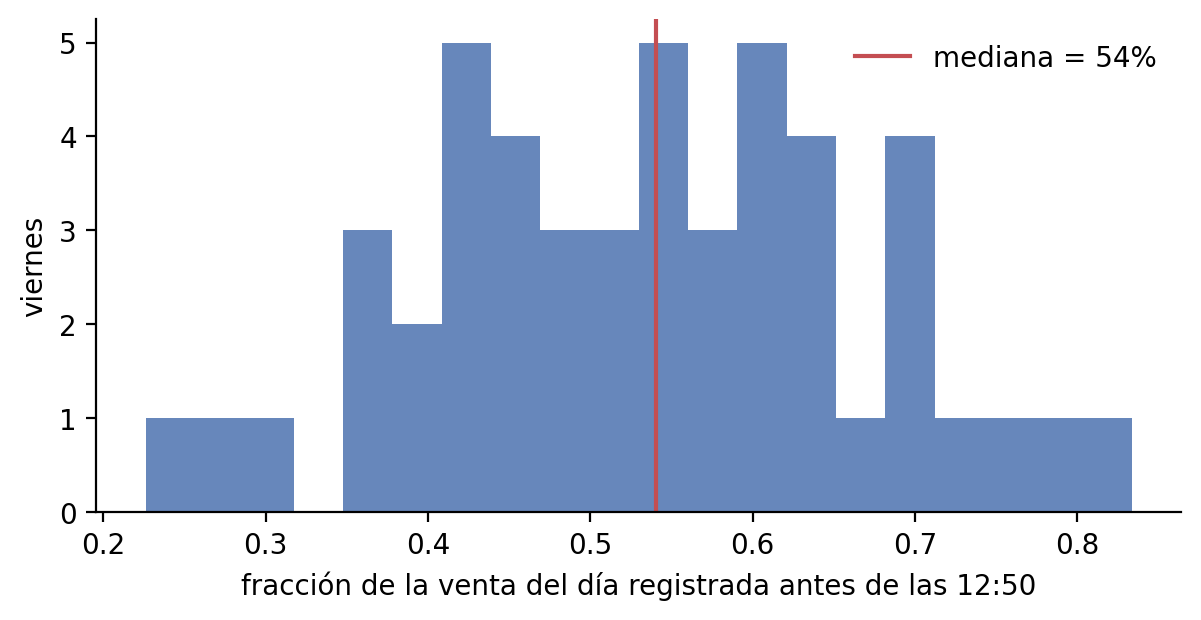
\includegraphics[width=0.7\textwidth]{p2_fraccion_corte.png}
  \caption{Fracción de la venta bruta de cada viernes registrada antes de las
  12:50, la hora de la última factura del 9 de diciembre.}
  \label{fig:p2_corte}
\end{figure}

Se descarta. Dejarlo metería en el último punto de la serie una caída
artificial a la mitad, justo en el día que más pesa al pronosticar, y es
también el día del par venta--cancelación de \pounds168\,470 del inciso 1.4.
Escalarlo por 1/0.54 inventaría un dato con un supuesto sobre el reparto de
las ventas en el día. Como es el último día y no hay nada que interpolar,
quitarlo no le cuesta nada a la serie. La serie de trabajo termina el jueves 8
de diciembre de 2011.
